\chapter{Evaluating the Calibrated Simulation at BER}
\label{ch:evaluation}

This chapter evaluates the pipeline on the BER data. It first checks the observations and the empirical properties derived from them, and then uses the simulation to answer the three research questions.

\section{Data Quality and Source Correspondence}
\label{sec:eval-data}

\subsection{Experimental Setup}
The A-CDM collection is checked for completeness per day and for agreement between its CSV, JSON and raw responses. Its actual takeoff times are compared with the OpenSky first observation of the same departure using the linkage rule of Section~\ref{sec:method-data}, under both the UTC and the Europe/Berlin interpretation of the naive A-CDM timestamps.

\subsection{Results}
Table~\ref{tab:acdmcoverage} shows the coverage. All 1,322 records passed the consistency checks. Of the 1,286 eligible actual takeoffs, 1,257 (97.7\%) have a unique OpenSky correspondence, and all of them support the UTC interpretation. The median absolute difference between OpenSky and A-CDM is 8~seconds; 1,237 matches agree within one minute and all 1,257 within five minutes. We therefore interpret the A-CDM timestamps as UTC in all further analyses.

\begin{table}[htbp]\centering\small
\begin{tabular}{lrrr}\hline
Date (2026) & Records & Eligible ATOT & Unique OpenSky match\\\hline
1 November & 289 & 283 & 280\\
5 November & 257 & 251 & 244\\
8 November & 264 & 250 & 243\\
15 November & 254 & 249 & 242\\
16 November & 258 & 253 & 248\\\hline
Total & 1,322 & 1,286 & 1,257\\\hline
\end{tabular}
\caption{A-CDM departure records and OpenSky correspondence per operational day.}
\label{tab:acdmcoverage}
\end{table}

For the 1,283 complete milestone triples, TSAT lies on average 1.30~minutes after TOBT (median 0), and ATOT 12.58~minutes after TSAT (median 12.12). Twenty-two triples violate the expected order $\mathrm{TOBT}\le\mathrm{TSAT}\le\mathrm{ATOT}$; they are retained but flagged. Because the board is retrieved once after the end of the day, only the last value of each target is available, and earlier values that might have respected the order are not.

\section{Empirical Turnaround Properties, Delay Drivers and Early Warning}
\label{sec:eval-props}

\subsection{Experimental Setup}
P1 and P2 are computed on the 610 linked turnarounds and P3 and P4 on the 1,283 complete departures. Associations are measured by Spearman's $\rho$ with 95\% bootstrap intervals from 5,000 resamples. The held-out delay-transfer model and the delay-driver models use the February--April data; the early-warning classifiers use both datasets (Section~\ref{sec:method-targets}).

\subsection{P1: Buffer-Dependent Delay Transfer}
When the inbound aircraft lands 30~minutes or less before the scheduled departure, the operator sets the TOBT more than five minutes after STD in 99\% of the cases, with a median shift of 35~minutes (Table~\ref{tab:p1}). Between 30 and 45~minutes of buffer this share falls to 53\%, and above 45~minutes it stays between 14\% and 26\%. The rank correlation between buffer and target shift is $\rho=-0.54$ (95\% CI $[-0.60,-0.46]$), and it is stable across days ($-0.52$, $-0.57$ and $-0.54$ on 1, 5 and 8~November).

\begin{table}[htbp]\centering\small
\begin{tabular}{lrrr}\hline
Scheduled buffer $B$ & $n$ & TOBT $>$ STD $+5$\,min & Median $\Delta^{\mathrm{TOBT}}$ (min)\\\hline
$\le 30$ min & 88 & 99\% & 35.0\\
30--45 min & 90 & 53\% & 7.5\\
45--60 min & 216 & 26\% & 0.0\\
60--90 min & 159 & 23\% & 0.0\\
$>90$ min & 57 & 14\% & 0.0\\\hline
\end{tabular}
\caption{P1: share of linked turnarounds with a late target off-block time by scheduled buffer, $n=610$.}
\label{tab:p1}
\end{table}

\subsection{P2: Target Turnaround Time}
The target turnaround time from the landing proxy to the TOBT differs clearly between carrier classes (Table~\ref{tab:p2}). Under time pressure, low-cost carriers plan turnarounds of 33.7~minutes or less in 5\% of the cases, full-service carriers 37.1~minutes. These distributions are the calibration targets of Section~\ref{sec:eval-rq1}.

\begin{table}[htbp]\centering\small
\begin{tabular}{llrrrr}\hline
Carrier class & Buffer & $n$ & 5th pct. & 25th pct. & Median\\\hline
Low-cost & $<45$ min & 113 & 33.7 & 39.7 & 44.7\\
Low-cost & $\ge45$ min & 163 & 41.9 & 51.3 & 61.0\\
Full-service/other & $<45$ min & 65 & 37.1 & 44.6 & 52.3\\
Full-service/other & $\ge45$ min & 269 & 47.7 & 55.4 & 64.0\\\hline
\end{tabular}
\caption{P2: target turnaround time (landing proxy to TOBT, minutes) by carrier class and schedule pressure.}
\label{tab:p2}
\end{table}

\subsection{P3 and P4: Runway Contention and Rotation Carry-Over}
The interval from start-up approval to takeoff grows with the number of other departures planned around the same time, from a median of 10.2~minutes with at most two others within $\pm15$~minutes ($n=27$) to 12.9~minutes with more than eight ($n=632$; $\rho=0.14$, CI $[0.08,0.19]$). In 154 cases, the same aircraft departed BER twice on one day; the departure delays of the two flights are positively associated ($\rho=0.27$, CI $[0.11,0.42]$).

\subsection{Delay Drivers and Weather}
On the February--April data, the outbound delay increases by 0.43~minutes per minute of inbound delay (95\% day-resampled CI $[0.13,0.62]$), and an inbound delay of more than 15~minutes doubles the odds of an outbound delay above 15~minutes (odds ratio 2.10, CI $[1.18,3.17]$). Low-cost turnarounds have lower odds of a late departure than full-service turnarounds (odds ratio 0.74, CI $[0.56,0.97]$), although their scheduled ground times are shorter (median 110 versus 145~minutes).

Weather shows the expected direction, but the evidence is weak. With precipitation at landing, 56\% of departures are more than 15~minutes late, compared with 45\% in dry conditions (median delay 18 versus 14~minutes). All eight turnarounds with gusts of 50~km/h or more departed late (median 36~minutes). In the multivariable model, however, the odds ratios for precipitation (1.25, CI $[0.72,2.95]$) and gusts of 40~km/h or more (3.09, with an unbounded upper limit) are not distinguishable from one, because the data cover only 20 days and few weather events. No de-icing conditions occurred in the observed periods.

\subsection{Held-Out Delay-Transfer Model}
Table~\ref{tab:heldout} reports the reactionary-delay model of Equation~\ref{eq:transfer}. On the April test data it is clearly better than assuming full transfer of the inbound delay, but it does not outperform a constant prediction. Only 9.8\% (full-service) and 16.5\% (low-cost) of the test turnarounds exceed the estimated slack, so the minimum turnaround time is poorly identified. Together with P1, this shows that inbound delay is transferred mainly when the buffer is short; with the long scheduled ground times of this sample, most outbound delay arises at BER itself.

\begin{table}[htbp]\centering\footnotesize
\begin{tabular}{lrrrrrr}\hline
& & & \multicolumn{3}{c}{Test MAE (min)} & \\\cline{4-6}
Class & $n_{\mathrm{train}}/n_{\mathrm{test}}$ & MTT [95\% CI] & Model & Full transf. & Const. & Slack exc.\\\hline
Full-service & 1,094 / 305 & 70 [20, 90] & 17.5 & 21.1 & 16.3 & 9.8\%\\
Low-cost & 390 / 278 & 62 [37, 80] & 18.7 & 22.9 & 18.2 & 16.5\%\\\hline
\end{tabular}
\caption{Held-out evaluation of the delay-transfer model (Eq.~\ref{eq:transfer}), trained on 21~February--4~March and tested on 17--24~April~2026.}
\label{tab:heldout}
\end{table}

\subsection{Early Warning at Landing}
Table~\ref{tab:earlywarning} shows that a late TOBT can be detected when the inbound aircraft lands. On each held-out November day, the classifiers reach an AUC between 0.76 and 0.82. When as many turnarounds are flagged as are actually late, 59--70\% of the flagged turnarounds are indeed late, compared with base rates of 33--48\%. The scheduled buffer is by far the most important feature (mean permutation importance 0.28 AUC), followed by temperature (0.02) and hour (0.01); the remaining weather variables, the carrier class and the arrival load contribute little. The median lead time, the scheduled buffer itself, is 54~minutes.

\begin{table}[htbp]\centering\footnotesize
\begin{tabular}{lrrrr}\hline
Test day & Base rate & AUC (logistic) & AUC (trees) & Precision\\\hline
1 November & 0.48 & 0.80 & 0.81 & 0.70\\
5 November & 0.33 & 0.82 & 0.76 & 0.59\\
8 November & 0.34 & 0.79 & 0.80 & 0.65\\\hline
Feb--Apr data (test April) & 0.35 & 0.54 & 0.53 & 0.42\\\hline
\end{tabular}
\caption{Early detection of delays at landing. November 2026: late TOBT, leave-one-day-out. February--April: outbound delay above 15 minutes, trained on February--March. Trees: gradient-boosted trees. Precision of the boosted trees when as many turnarounds are flagged as are actually late (base rate).}
\label{tab:earlywarning}
\end{table}

On the February--April data, predicting the actual outbound delay at landing does not work (AUC 0.53--0.54). The actual delay depends on events after landing that these features do not capture, and the flight-number pairing may join flights that are not true rotations. Early warning is therefore feasible for the \emph{planned} target, which depends strongly on the buffer, but not yet for the \emph{actual} departure delay.

\subsection{Disruption Screening}
Screening the 41 days of OpenSky turnarounds against a season- and weekday-specific baseline flags 15--17 and 20~October, when the median ground time of short stays was about 5--9~minutes above normal ($z$ between 3.2 and 5.6). These days were dry and calm (maximum gusts below 35~km/h), so weather does not explain them. They coincide with the start of the Berlin and Brandenburg autumn school holidays on 19~October~\cite{herbstferien2026}, when fuller flights and more baggage can lengthen turnarounds. In early November, the screening also flags a day with low traffic (8~November) and one with long ground times (9~November), but the winter-schedule baseline contains only 16 days and is less reliable. Larger disruptions, such as the warning strike that closed BER on 18~March~2026~\cite{aerointernational2026streik}, fall outside the collected periods; with no turnarounds at all, such a day would be flagged immediately.

\section{Simulation Integrity and Run-to-Run Variability}
\label{sec:eval-integrity}

All 499 simulation runs reported in this chapter (three timing configurations and six what-if scenarios on 41 days, the 116 runs of the calibration grid and 14 validation runs on the held-out days) completed and passed the automatic checks: every released turnaround departed, all aircraft and resource tokens returned to their pools, and all metrics were finite and nonnegative. The exported logs contain no dangling event-to-object or object-to-object references. One modeling artefact remains: some resource objects are related to service events twice, once with the qualifier of the resource and once with the qualifier \texttt{turnaround}.

The Monte Carlo comparison quantifies how much a single run of a day can vary. With ten independent replications per scenario on 1 and 8~November, the 95\% interval of the mean block duration is between $\pm0.3$ and $\pm1.7$~minutes. This is small compared with the effects studied below and with the variation between days, which justifies single trace-driven runs per day and the use of the day as the statistical unit.

\section{RQ1: Calibration of Service Times}
\label{sec:eval-rq1}
\label{sec:eval-validity}

\subsection{Experimental Setup}
For every linked turnaround, the simulated time from arrival release to \emph{Aircraft Ready} is compared with the observed target turnaround time (P2). We first compare the three timing configurations on all 41 days, then calibrate the carrier-specific configuration (Section~\ref{sec:method-calibration}).

\subsection{Timing Configurations}
Table~\ref{tab:timingconfig} shows that the carrier-specific service times reproduce the observed targets far better than the original and the carrier-agnostic literature functions. For low-cost turnarounds, the mean quantile error drops from 13.5~minutes (original) and 10.6~minutes (literature) to 5.8~minutes; for full-service turnarounds from 10.8 and 4.5~minutes to 3.8~minutes. The comparison also revealed that leisure carriers do not behave like low-cost carriers: their observed target turnaround is long (median 79.8~minutes), and the low-cost profile underestimates it by more than 27~minutes. Leisure carriers therefore use the full-service profile in the calibrated model.

\begin{table}[htbp]\centering\small
\begin{tabular}{lrrr}\hline
Mean quantile error (min) & Original & Literature & Carrier-specific\\\hline
Full-service ($n=259$) & 10.8 & 4.5 & 3.8\\
Low-cost ($n=266$) & 13.5 & 10.6 & 5.8\\
Leisure ($n=52$), low-cost profile & 10.8 & 13.8 & 27.7\\\hline
\end{tabular}
\caption{Mean absolute difference of the 5th, 25th, 50th and 75th percentiles between simulated arrival-to-ready time and observed target turnaround time, linked turnarounds, one run per day.}
\label{tab:timingconfig}
\end{table}

\subsection{Calibration and Held-Out Validation}
The grid search places the optimum at $s_{\mathrm{LCC}}=1.3$ and $s_{\mathrm{FSC}}=1.1$ (calibration loss 2.03~minutes, compared with 4.84~minutes without calibration). Neighbouring values are clearly worse, and extending the grid to $s_{\mathrm{LCC}}=1.6$ confirmed that the optimum is interior. The literature service times are therefore slightly too fast for BER, by about 30\% for low-cost and 10\% for full-service turnarounds.

The calibration is validated on three held-out days that were not used for fitting: 8~November and the two most recent collection days, 15 and 16~November. The latter lie outside the frozen 41-day period; their 437 turnarounds were reconstructed from the raw OpenSky lists with the same pairing rule and linked to A-CDM in the same way (372 linked low-cost and full-service turnarounds). Table~\ref{tab:calibration} compares the calibrated model with the uncalibrated carrier timing, the carrier-agnostic literature timing and the original timing.

On 8~November, calibration reduces the loss from 8.55 to 2.39~minutes. The simulated low-cost quartiles move from $[36.8, 44.9, 53.3]$ to $[43.1, 52.1, 59.8]$~minutes against observed $[44.5, 52.6, 66.1]$, and the full-service quartiles from $[45.3, 55.2, 67.6]$ to $[51.9, 60.6, 72.6]$ against observed $[55.3, 63.1, 72.9]$. On 15--16~November the reduction is smaller, from 6.05 to 3.85~minutes. Here the full-service turnarounds are reproduced closely (median 59.4 against 59.1~minutes), but the low-cost turnarounds remain about six minutes too fast at the 25th and 50th percentiles.

The comparison with the literature timing is more nuanced. On 8~November the calibrated model is clearly better (2.39 against 6.59~minutes), whereas on 15--16~November both reach the same overall loss (3.85 and 3.82). The errors have opposite signs: the carrier-agnostic literature timing makes low-cost turnarounds too \emph{slow} on all three days (by 4 to 14~minutes per quartile), while the calibrated model makes them slightly too \emph{fast} on 15--16~November. Averaged over the two held-out sets, the calibrated model has the lowest loss (3.1~minutes, against 5.2 for literature, 7.3 for uncalibrated and 8.7 for original timing). The calibration therefore generalizes in direction and order of magnitude, while the remaining differences of a few minutes between days are larger than the run-to-run variability (Section~\ref{sec:eval-integrity}) and indicate genuine day-to-day variation in the planned turnaround times.

\begin{table}[htbp]\centering\small
\begin{tabular}{llccr}\hline
Held-out day(s) & Source & Low-cost quartiles & Full-service quartiles & Loss\\\hline
8 Nov. & observed TTA & $[44.5, 52.6, 66.1]$ & $[55.3, 63.1, 72.9]$ & \\
 & calibrated & $[43.1, 52.1, 59.8]$ & $[51.9, 60.6, 72.6]$ & \textbf{2.39}\\
 & uncalibrated & $[36.8, 44.9, 53.3]$ & $[45.3, 55.2, 67.6]$ & 8.55\\
 & literature & $[52.4, 66.2, 76.1]$ & $[49.0, 63.1, 74.6]$ & 6.59\\
 & original & $[57.4, 67.3, 85.2]$ & $[57.4, 73.0, 82.8]$ & 11.43\\\hline
15--16 Nov. & observed TTA & $[44.0, 51.3, 65.4]$ & $[52.0, 59.1, 68.5]$ & \\
 & calibrated & $[38.3, 45.5, 61.4]$ & $[47.2, 59.4, 71.1]$ & 3.85\\
 & uncalibrated & $[36.0, 47.7, 56.0]$ & $[44.6, 53.9, 65.7]$ & 6.05\\
 & literature & $[48.7, 59.1, 69.8]$ & $[47.6, 58.8, 67.2]$ & \textbf{3.82}\\
 & original & $[49.9, 58.8, 67.7]$ & $[57.0, 67.4, 75.5]$ & 6.02\\\hline
\end{tabular}
\caption{Held-out validation of the calibration (minutes; 25th, 50th and 75th percentiles of the target turnaround time). 8~November: 88 low-cost and 100 full-service linked turnarounds; 15--16~November: 174 and 198.}
\label{tab:calibration}
\end{table}

\subsection{Validation on the 41-Day Demand}
On all 41 days, the calibrated model also reproduces the ground intervals of the 10,212 OpenSky turnarounds at the lower and middle quantiles. For short stays of full-service aircraft, the simulated 25th and 50th percentiles of the arrival-to-takeoff time are 64.1 and 75.6~minutes against observed 64.2 and 71.6; for low-cost aircraft 56.0 and 65.6 against 57.2 and 66.6. The original timing overestimates these quantiles by 10 to 14~minutes. The upper tail is not reproduced, because most simulated aircraft without a linked schedule depart as soon as they are ready.

Figure~\ref{fig:p1sim} compares the simulated delay-transfer curve with the observed one. Under schedule binding, the simulated share of late targets equals $\max(0,\mathrm{ready}-\mathrm{STD})>5$~minutes. The calibrated model reproduces the observed transfer at short buffers and moves the 30--45-minute class from 99\% (original) to 78\% (observed 54\%). It still transfers too much delay at intermediate buffers, because it does not compress turnarounds under pressure.

\begin{figure}[htbp]
\centering
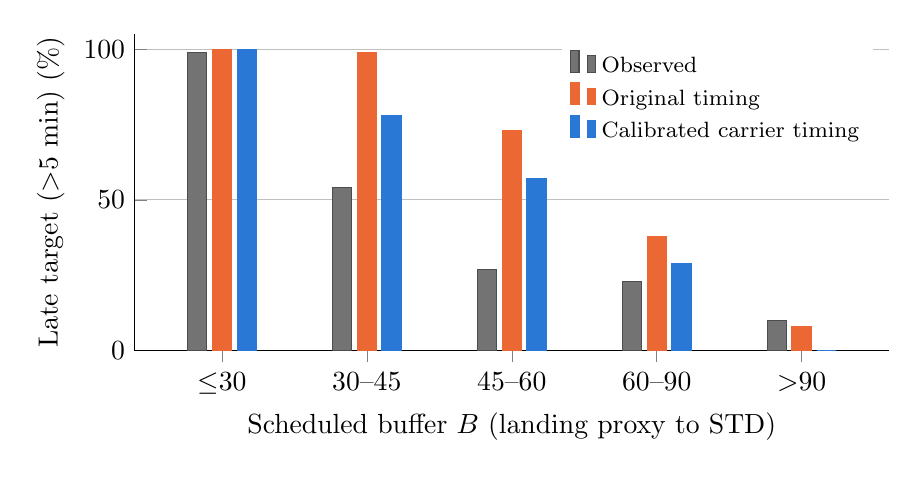
\begin{tikzpicture}
\begin{axis}[
  ybar, bar width=7pt, width=0.92\textwidth, height=5.6cm,
  ymin=0, ymax=105, ylabel={Late target ($>$5 min) (\%)},
  xlabel={Scheduled buffer $B$ (landing proxy to STD)},
  symbolic x coords={{$\le$30},{30--45},{45--60},{60--90},{$>$90}},
  xtick=data, enlarge x limits=0.15, axis lines*=left, ymajorgrids,
  legend style={at={(0.98,0.97)}, anchor=north east, font=\footnotesize, draw=none}, legend cell align=left]
\addplot[fill=black!55, draw=black!70] coordinates {({$\le$30},99) ({30--45},54) ({45--60},27) ({60--90},23) ({$>$90},10)};
\addplot[fill={rgb,255:red,235;green,104;blue,52}, draw={rgb,255:red,235;green,104;blue,52}] coordinates {({$\le$30},100) ({30--45},99) ({45--60},73) ({60--90},38) ({$>$90},8)};
\addplot[fill={rgb,255:red,42;green,120;blue,214}, draw={rgb,255:red,42;green,120;blue,214}] coordinates {({$\le$30},100) ({30--45},78) ({45--60},57) ({60--90},29) ({$>$90},0)};
\legend{Observed, Original timing, Calibrated carrier timing}
\end{axis}
\end{tikzpicture}
\caption{Observed and simulated delay-transfer curves (P1) for the linked turnarounds.}
\label{fig:p1sim}
\end{figure}

\section{RQ2: Waiting, Synchronization and Delay Propagation}
\label{sec:eval-promenade}

\subsection{Experimental Setup}
We analyze the calibrated reference runs of all 41 days by carrier class and stand type, and the calibrated event logs of 1, 5 and 8~November with PM4Py and Promenade (Section~\ref{sec:method-ocel}).

\subsection{Which Branch Determines Readiness}
Table~\ref{tab:mechanism} shows which handling branch finishes last at the join. For full-service turnarounds, the cabin and boarding branch is last in 86\% of the cases. For low-cost turnarounds, whose cabin services are shorter, it is last in only 76\%, and the baggage hold becomes the critical branch in 13\% of the cases, compared with 3\% for full-service. Faster cabin processes thus shift the bottleneck to the ramp.

\begin{table}[htbp]\centering\small
\begin{tabular}{lrrrrr}\hline
Class & Turnarounds & Cabin/boarding & Baggage hold & Fuel & Other\\\hline
Full-service & 3,993 & 86.2\% & 3.4\% & 8.7\% & 1.7\%\\
Leisure & 928 & 87.2\% & 2.4\% & 9.2\% & 1.2\%\\
Low-cost & 4,963 & 76.4\% & 12.9\% & 6.8\% & 3.9\%\\\hline
Contact stands & & 70.8\% & 12.7\% & 12.0\% & 4.5\%\\
Remote stands & & 99.0\% & 0.0\% & 1.0\% & 0.0\%\\\hline
\end{tabular}
\caption{Last-ready handling branch in the calibrated reference runs (41 days), by carrier class and stand type.}
\label{tab:mechanism}
\end{table}

\subsection{Terminal and Remote Stands}
Remote stands, which receive 38\% of the turnarounds in the model, add 18.5~minutes to the time until the aircraft is ready (paired daily difference, 95\% CI $[17.0,20.0]$) and 17.8~minutes to the block time ($[16.3,19.3]$). On remote stands, deplaning and boarding by bus make the cabin branch the last-ready branch in 99\% of the turnarounds; on contact stands, the bottleneck is spread over cabin (71\%), baggage (13\%) and fuel (12\%). Within each carrier class, the median ready time is about 19~minutes longer on a remote stand (low-cost 59.3 versus 40.9~minutes, full-service 68.6 versus 48.9~minutes). These values describe the mechanism, not BER's actual remote-stand penalty. BER does not publish its stand layout, the walking and driving distances to its remote stands or the size of its bus fleet, so the model keeps the stand geometry and the bus fleet of the generic baseline airport. The size of the penalty therefore depends on these inherited assumptions, while its cause, bus transport on the cabin branch, does not.

\subsection{Object-Centric Process Discovery}
The calibrated log of 8~November contains 8,914 events, 1,104 objects and 47 activities. Figure~\ref{fig:ocdfg} shows the OC-DFG restricted to the shared resources. Each color stands for one resource type, each node for an activity, and each edge for a directly-follows relation of objects of that type, labeled with how often it occurs. Unlike a turnaround, a resource object does not have a single start and end: it returns to an earlier activity when it serves the next aircraft, so its edges form cycles. The figure makes the lifecycle of each resource across turnarounds visible: pushback tugs cycle through \emph{attached}, \emph{start-up} and \emph{off-block}; fuel tankers alternate between \emph{dispatch}, \emph{refuelling} and, 30 times on this day, \emph{reload at depot}; buses run deplaning and boarding cycles; and loaders move between unloading and loading of different aircraft. None of these cycles is visible in a case-centric log of turnarounds.

\begin{figure}[htbp]\centering
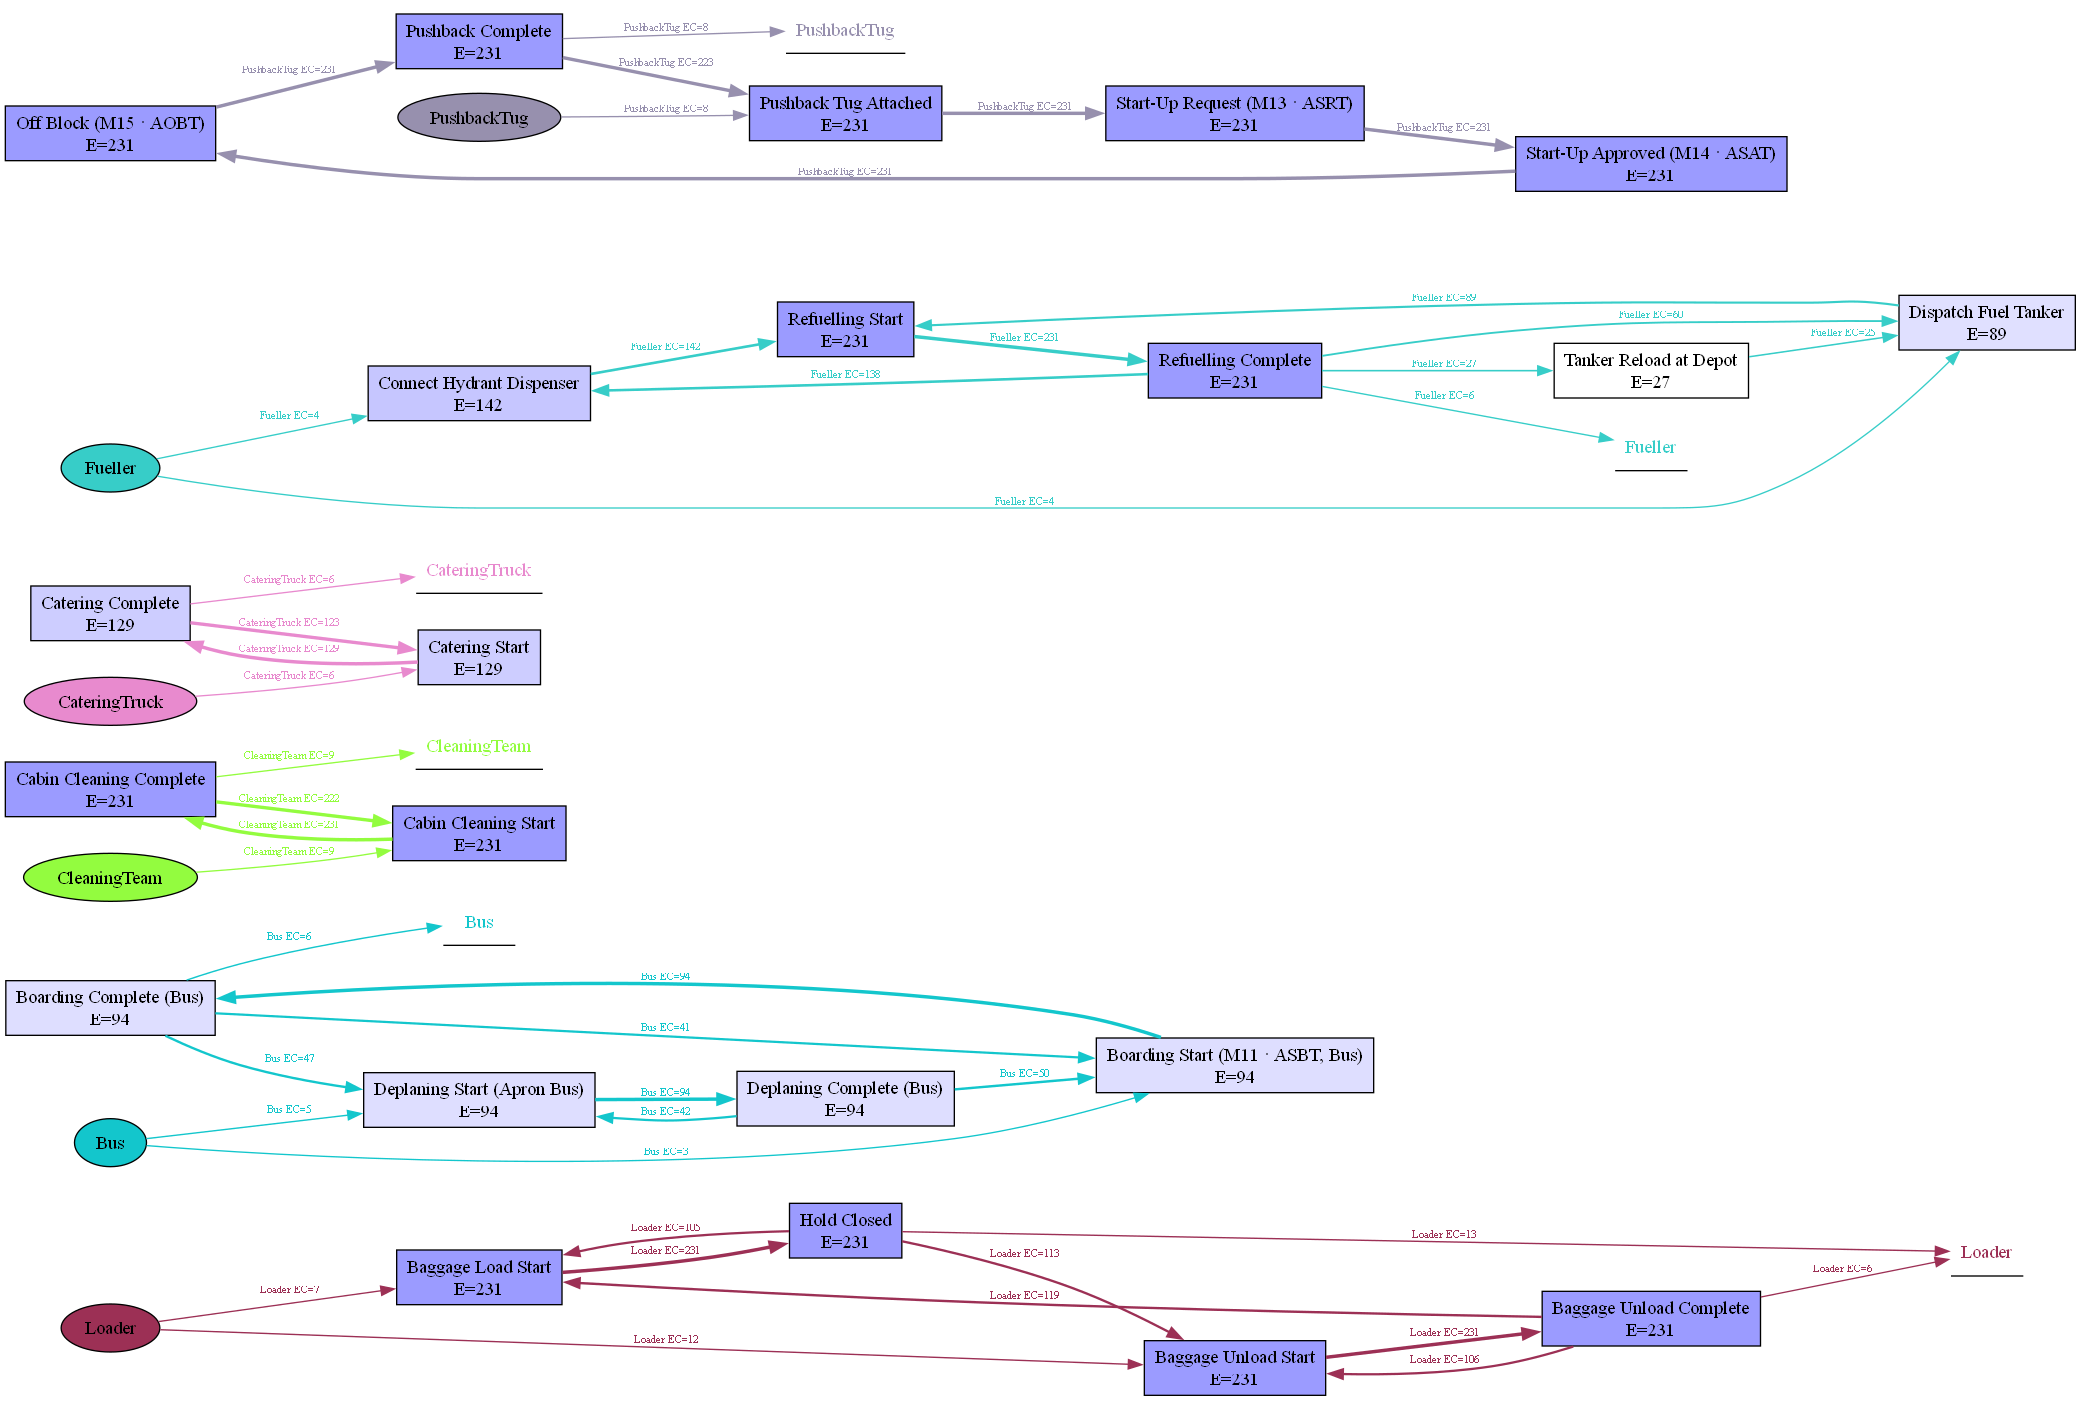
\includegraphics[width=\textwidth]{pm_ocdfg_resources.png}
\caption{OC-DFG of the shared resource types discovered with PM4Py from the calibrated log of 8 November (edge labels: event couples).}
\label{fig:ocdfg}
\end{figure}

The discovered OCPN (Figure~\ref{fig:ocpn}) shows the turnaround in brown and three resource types in color: fuel tankers and buses in cyan and cleaning teams in green. Read from top to bottom, the brown part recovers the sequential parts of the turnaround (approach, in-block, pushback, taxi-out), and the colored parts at the bottom recover the resource cycles. The parallel handling between \emph{Start Ground Handling} and \emph{Aircraft Ready}, however, is represented as a single place in the middle of the figure from which all handling activities can occur in any order and any number of times (a so-called flower structure). The reason is concurrency: among 383 full-service and 330 low-cost turnarounds of the three days, 381 and 318 have a unique order of activities, so the inductive miner finds no order that holds for all of them.

\begin{figure}[htbp]\centering
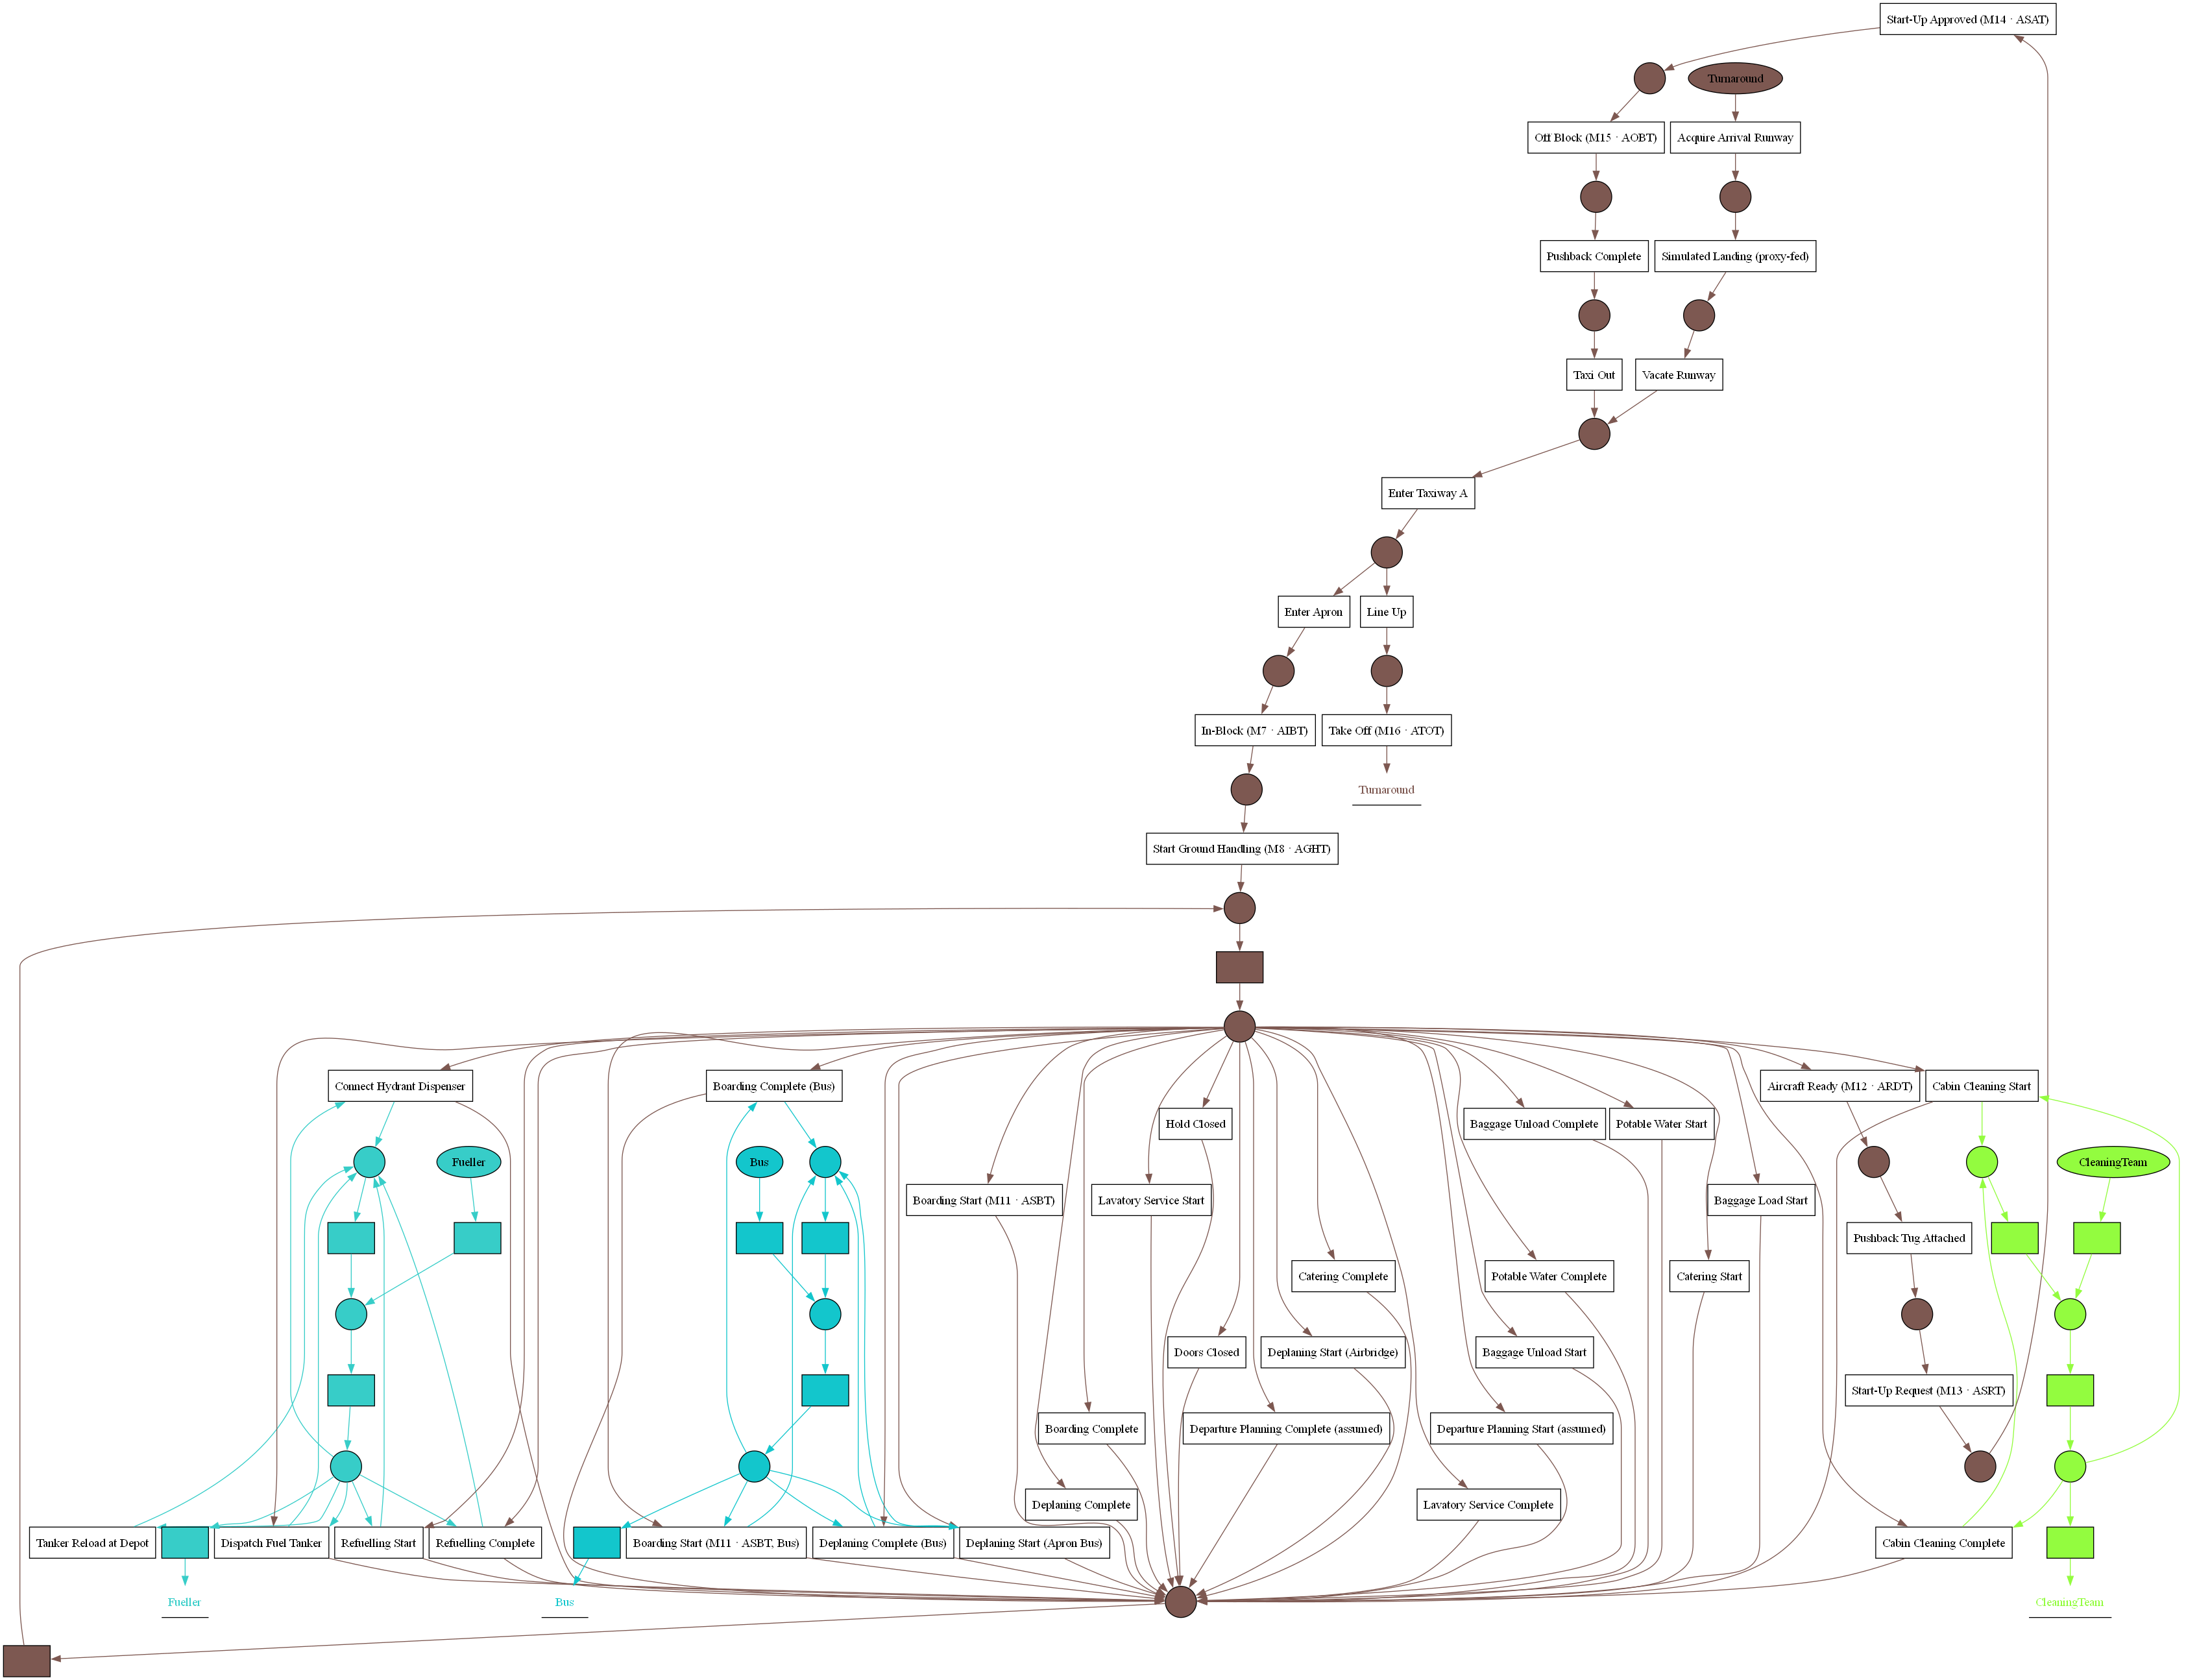
\includegraphics[width=\textwidth]{pm_ocpn.png}
\caption{OCPN discovered with PM4Py (inductive miner) for the object types Turnaround, Fueller, Bus and CleaningTeam.}
\label{fig:ocpn}
\end{figure}

\subsection{Carrier-Specific Behavior in the Event Logs}
Flattening the logs on the turnaround object confirms the carrier differences at the level of the individual services (Table~\ref{tab:pmdurations}). Cleaning, catering and boarding take 5--7~minutes less for low-cost turnarounds, and the median ground handling from its start to \emph{Aircraft Ready} is 36.2 versus 48.6~minutes.

\begin{table}[htbp]\centering\small
\begin{tabular}{lrrrr}\hline
Service (median, min) & Full-service & Low-cost & Full p90 & Low p90\\\hline
Deplaning & 7.5 & 8.1 & 16.3 & 17.2\\
Cleaning & 15.5 & 10.1 & 21.5 & 16.2\\
Catering & 18.3 & 11.6 & 29.6 & 16.4\\
Refuelling & 14.2 & 14.8 & 34.6 & 23.9\\
Boarding & 20.2 & 14.0 & 29.7 & 23.6\\
Ground handling (start to ready) & 48.6 & 36.2 & 65.0 & 55.0\\\hline
\end{tabular}
\caption{Service durations measured in the flattened calibrated logs (1, 5 and 8 November; 383 full-service and 330 low-cost turnarounds), including access and travel times.}
\label{tab:pmdurations}
\end{table}

Conformance checking makes the behavioral difference measurable. A natural reference would be the de-jure model, that is, the simulation model itself. Since every generated trace is produced by that model, replaying the logs on it would trivially yield perfect fitness and would show nothing. We therefore use the two carrier classes as references for each other: a model discovered from one class is replayed on the traces of both classes, and the fit on its own class serves as the baseline for the fit on the other class (Table~\ref{tab:conformance}). A Petri net discovered from low-cost turnarounds replays 82.7\% of the low-cost traces perfectly but only 65.5\% of the full-service traces; the net discovered from full-service turnarounds replays 61.4\% of full-service and 46.7\% of low-cost traces. Log fitness stays high (0.98--1.00) in all cases, whereas precision is low (0.26--0.29) because the discovered nets allow the parallel activities in any order.

\begin{table}[htbp]\centering\small
\begin{tabular}{llrrr}\hline
Model discovered from & Replayed log & Fitness & Perfectly fitting traces & Precision\\\hline
Low-cost & Low-cost & 0.997 & 82.7\% & 0.26\\
Low-cost & Full-service & 0.993 & 65.5\% & 0.26\\
Full-service & Full-service & 0.991 & 61.4\% & 0.29\\
Full-service & Low-cost & 0.984 & 46.7\% & 0.28\\\hline
\end{tabular}
\caption{Token-based replay conformance between carrier classes (flattened calibrated logs, inductive miner with noise threshold 0.2).}
\label{tab:conformance}
\end{table}

\subsection{Analysis in Promenade}
\todo[inline]{Figs.~6.4 and 6.5: retake the Promenade screenshots in light mode and crop them to the relevant part (supervisor comment).}
The Promenade performance spectrum of the calibrated 8~November log (Figure~\ref{fig:spectrum}) shows the slowest 25\% of flows concentrated in three segments: the wait from \emph{Aircraft Ready} to the start-up request of aircraft held to their schedule, the transition from baggage unloading to loading, and a departure that the night restriction holds until the morning. The process friction topography (Figure~\ref{fig:friction}), which raises each activity by its median waiting time, places its summit at \emph{Hold Closed} with a median queue of 4.7~minutes. This confirms the baggage hold as the main point of friction in the calibrated model.

\begin{figure}[htbp]\centering
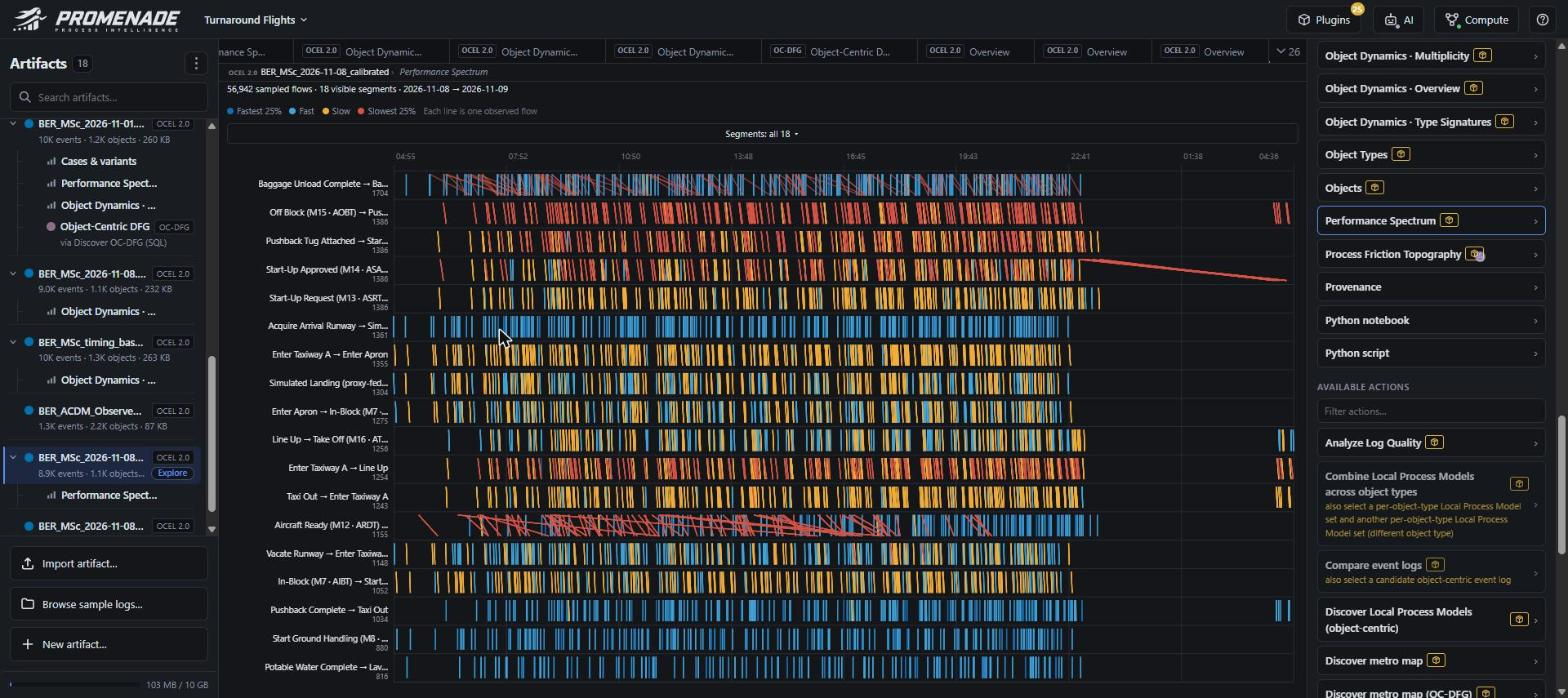
\includegraphics[width=\textwidth]{promenade_performance_spectrum.jpg}
\caption{Promenade performance spectrum of the calibrated log of 8 November (blue: fastest flows, red: slowest 25\%).}
\label{fig:spectrum}
\end{figure}

\begin{figure}[htbp]\centering
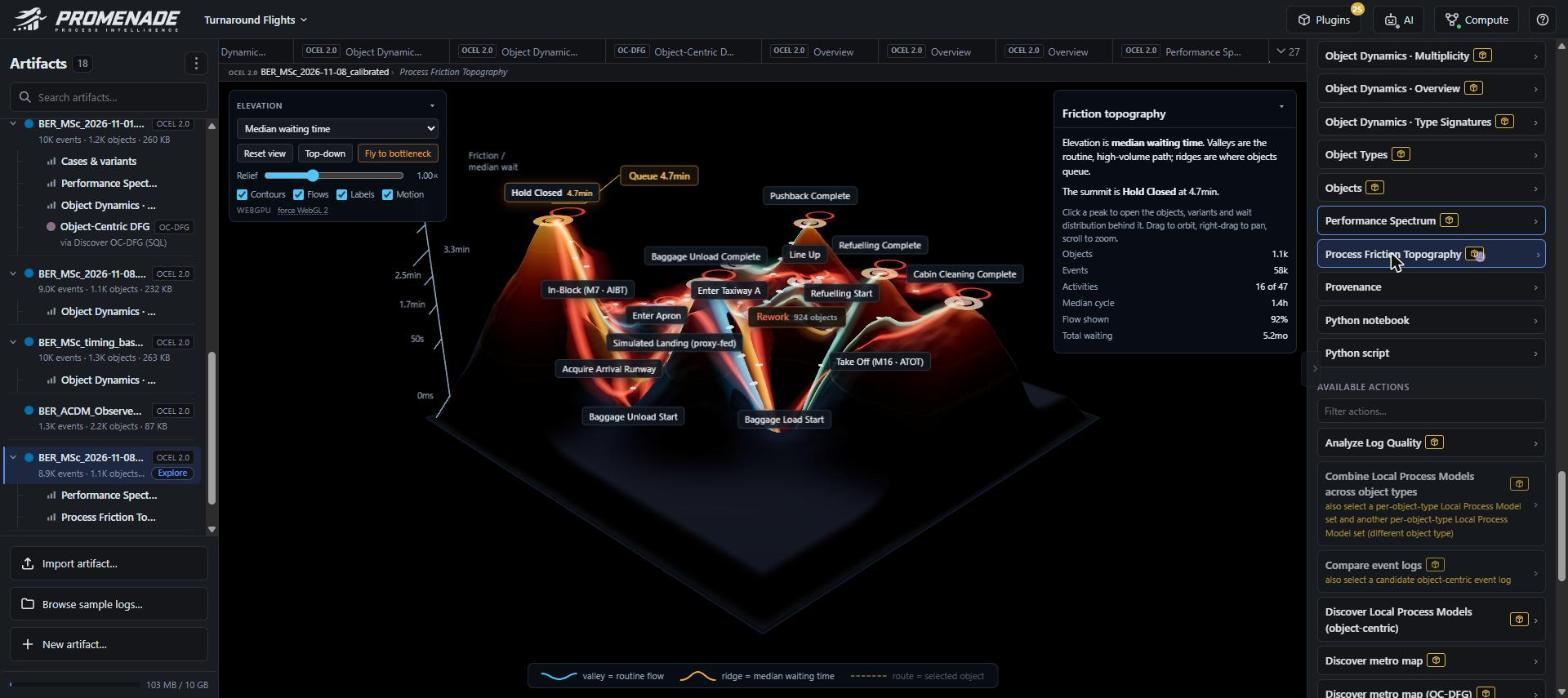
\includegraphics[width=\textwidth]{promenade_friction_topography.jpg}
\caption{Promenade process friction topography of the calibrated log of 8 November; elevation is the median waiting time.}
\label{fig:friction}
\end{figure}

Finally, Promenade's event-log comparison between the calibrated and the original-timing log of the same day finds identical behavior and objects at the type level: all 47 activity types are shared, and 94.5\% of the objects. Only 63.7\% of the events coincide, because their timestamps differ. Calibration thus changes \emph{when} the services happen, not \emph{which} services happen.

\subsection{Delay Propagation in the Simulation}
Delay propagates in the model through the same three channels as in the observations: through the turnaround, as the simulated transfer curve shows (Figure~\ref{fig:p1sim}); through the aircraft, whose token is reused in later rotations of the day, as the running example shows; and through shared resources, whose queues (fuel dispatch, pushback tugs) delay the branches that use them. The object-centric view separates waiting that matters from waiting that does not: an aircraft can wait for fuel without any effect on its readiness if its cabin branch finishes later.

\section{RQ3: Resource and Allocation Scenarios}
\label{sec:eval-whatif}

\subsection{Experimental Setup}
The calibrated model is run on all 41 days for the reference and five scenarios (Section~\ref{sec:method-calibration}). Effects are paired daily differences with 95\% Student-$t$ intervals over 41 days.

\subsection{Results}
Table~\ref{tab:whatif} and Figure~\ref{fig:whatif} summarize the effects on the time from arrival to \emph{Aircraft Ready}, whose reference mean is 58.7~minutes. Faster boarding is the most effective single lever: a 15\% reduction of boarding time shortens the time to readiness by 2.2~minutes and the block time by 1.5~minutes, and it benefits full-service turnarounds most ($-2.6$~minutes), because their cabin branch is critical more often. Additional fuel capacity removes almost the whole fuel queue ($-2.5$~minutes of dispatch waiting) but shortens the time to readiness by only 1.3~minutes, more for low-cost ($-1.8$) than for full-service turnarounds. Four additional buses shorten the time to readiness by about half a minute, and five additional loaders do not change it; for both, the confidence interval includes zero.

\begin{table}[htbp]\centering\footnotesize\setlength{\tabcolsep}{4pt}
\begin{tabular}{lrrr}\hline
Scenario (vs.\ calibrated reference) & Ready (min) & Block (min) & Fuel wait (min)\\\hline
Boarding 15\% faster & $-2.17$ [$-2.85$, $-1.49$] & $-1.50$ [$-2.06$, $-0.94$] & $+0.30$ [$-0.12$, $+0.71$]\\
Fuel 6+6 instead of 4+4 & $-1.35$ [$-2.10$, $-0.59$] & $-0.86$ [$-1.49$, $-0.22$] & $-2.47$ [$-2.83$, $-2.10$]\\
Buses 12 instead of 8 & $-0.56$ [$-1.19$, $+0.08$] & $-0.46$ [$-1.09$, $+0.16$] & $-0.29$ [$-0.64$, $+0.06$]\\
Loaders 24 instead of 19 & $-0.02$ [$-0.66$, $+0.63$] & $-0.19$ [$-0.80$, $+0.41$] & $+0.18$ [$-0.22$, $+0.58$]\\
Low-cost to remote stands & $+37.9$ [$+31.1$, $+44.7$] & $+7.1$ [$+5.4$, $+8.7$] & $-0.63$ [$-0.96$, $-0.30$]\\\hline
\end{tabular}
\caption{What-if effects: paired daily differences over 41 days with 95\% intervals.}
\label{tab:whatif}
\end{table}

\begin{figure}[htbp]
\centering
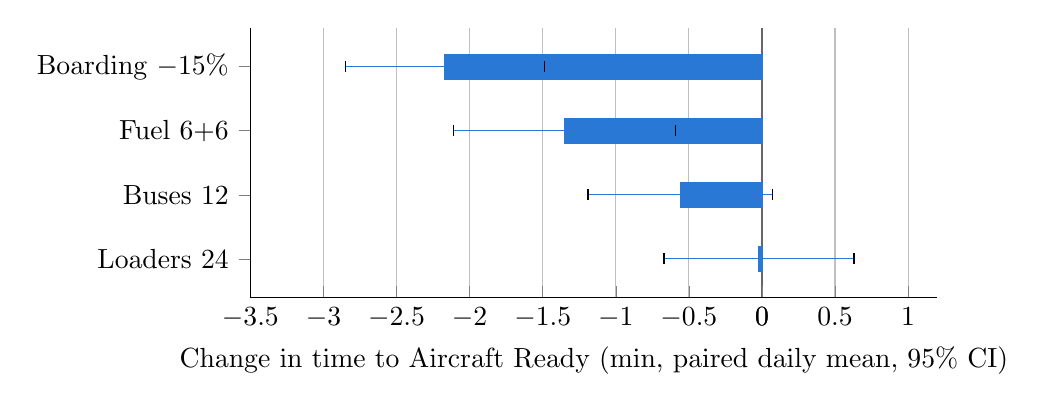
\begin{tikzpicture}
\begin{axis}[
  xbar=0pt, width=0.85\textwidth, height=5.0cm, xmin=-3.5, xmax=1.2,
  xlabel={Change in time to Aircraft Ready (min, paired daily mean, 95\% CI)},
  symbolic y coords={Loaders 24,Buses 12,Fuel 6+6,Boarding $-$15\%}, ytick=data,
  axis lines*=left, xmajorgrids, bar width=9pt, enlarge y limits=0.2,
  extra x ticks={0}, extra x tick style={grid=major, major grid style={black!60}}]
\addplot[fill={rgb,255:red,42;green,120;blue,214}, draw={rgb,255:red,42;green,120;blue,214},
  error bars/.cd, x dir=both, x explicit]
  coordinates {(-0.02,Loaders 24) +- (0.65,0) (-0.56,Buses 12) +- (0.63,0) (-1.35,Fuel 6+6) +- (0.76,0) (-2.17,Boarding $-$15\%) +- (0.68,0)};
\end{axis}
\end{tikzpicture}
\caption{Effects of capacity and process scenarios on the time to readiness. The allocation scenario (+37.9 min) is omitted for scale.}
\label{fig:whatif}
\end{figure}

The allocation strategy that sends all low-cost turnarounds to remote stands is clearly harmful in the modeled airport. Full-service turnarounds gain 9.0~minutes ($[-11.2,-6.8]$) from the freed contact stands, but low-cost aircraft wait for a free remote stand and need 86.8~minutes longer ($[73.3,100.3]$) until they are ready. The remote apron of the model is not large enough for the low-cost share of BER's demand. The strategy would only be viable with more remote stands or a flexible assignment that uses contact stands when the remote apron is full.

\section{Threats to Validity}
\label{sec:threats}

The results of this chapter rest on observations that were not collected for this purpose and on a model that was not built for BER. Both limit what the results can show. We discuss the threats in the order of the pipeline, from the data to the model and its runs.

The first threat concerns what the data measure. OpenSky's last observation of an arriving aircraft is only a proxy for its landing, and the A-CDM board is retrieved once after the end of the day, so only the last value of each target is available. The calibration therefore matches \emph{planned} turnaround times (TOBT) rather than actual ones, and these times include taxi-in. The data also contain few weather events and no de-icing conditions, so weather effects could not be estimated precisely, and the disruption screening relies on a short baseline. The carrier classification is based on business models, and the February--April records pair flights by flight number rather than by aircraft.

The second threat concerns the calibration. It uses two days and is validated on three held-out days with 560 linked turnarounds. On 15--16~November it does not improve on the carrier-agnostic literature timing, and low-cost turnarounds are simulated too fast. Leisure carriers ($n=52$) remain poorly reproduced (mean quantile error 11.8~minutes). The carrier-specific distributions themselves were measured at other airports and are scaled, not re-estimated, for BER, because individual service durations at BER are not observed.

The third threat concerns the model and its runs. Stand geometry and the bus, loader and fuel fleets are inherited from the generic airport model, because BER's infrastructure data are not public. Absolute effects of capacity and stand scenarios are therefore model-specific; their direction and relative size are the transferable result. Finally, each scenario is run once per day. The Monte Carlo comparison shows that the run-to-run variability is small, but individual days remain single realizations.

\section{Summary}

The evaluation shows that public milestones, once linked to arrival observations, reveal systematic properties of BER turnarounds and allow an early warning at landing with an AUC of about 0.8. Carrier-specific service times reproduce the observed targets far better than carrier-agnostic ones, and calibrating them by 30\% (low-cost) and 10\% (full-service) reduces the error on three held-out days by 36--72\%. The object-centric analysis shows that the cabin branch determines readiness for most turnarounds, that the baggage hold becomes critical for low-cost turnarounds, and that remote stands add almost 20~minutes. Process discovery and conformance checking make the carrier differences measurable in the event logs. Among the tested levers, faster boarding is most effective, additional fuel capacity mainly removes the fuel queue, and assigning all low-cost flights to remote stands overloads the remote apron.
